\cotefile{142}

\scanpage{77}
\mspage{6}
or tout chemin effectif $x\longrightarrow y$ (donné par une appl continue $[0,1]\longrightarrow X$) se décompose en \inserted{composé de} chemins \inserted{``directs''}
\diagram{\begin{tikzcd}[ampersand replacement=\&,column sep=small]
x_0=x \arrow[r] \& x_1 \arrow[r] \& x_2\,\mathord{-}\,\mathord{-} \arrow[r] \& x_n=y
\end{tikzcd}}
entre \deleted{chemins} \inserted{points} ``proches''. Dans le cas \deleted{général} \inserted{où les $X_\alpha$ sont fermés}, un argument de descente (comme déjà signalé dans la première hypothèse) donne le résultat énoncé.

Cette deuxième démonstration a l'avantage de marcher également pour \inserted{montrer} le résultat un peu plus général, et peut-être plus intéressant du point de vue pratique, où pour tt $\alpha$ on a $I_\alpha\subset T_\alpha$ partie \inserted{non vide} de $T_\alpha$ (normalement, partie finie) de telle façon que pour $T_\alpha\subset T_\beta$ on ait $I_\alpha\subset I_\beta$ \unsure{et|,} (normalement, on prend d'abord $I\subset X_K$ convenable et on prend $I_\alpha=I\cap T_\alpha$, donc $I=\bigcup I_\alpha$), et on se borne aux $g^\alpha_{y,x}$ pour $x,y\in I_\alpha$: leur connaissance permet de retrouver \uline{tous} \inserted{$f_l(u)$,} $g_{\deleted{\unsure{yx}}l}(u)$, $l$ un chemin quelconque dans

\margin{On a deux façons de ``récupérer'' l'opération de $\Gamma$ sur le groupoïde $\widehat{\Pi}_1(X,I)$ (où $I\subset X_K$) en quelque sorte duales l'une de l'autre: soit on prend un syst. de $l_j:x_j\mathbin{-}y_j$ $(x_j,y_j\in I)$ générateurs pour $\Pi_1(X,I)$, et regarde les $f_{l_j}(u)$ ou $g_{l_j}(u)$, soit on fixe des $T_\alpha$ comme dessus, et on regarde les $g^\alpha_{x,y}$ $(\alpha\in A,x,y\in T_\alpha\cap I)$. En fait on voit très bientôt qu'il est \deleted{\unsure{ff}} inutile de supposer que les $T_\alpha$ recouvrent $X$ (p.ex. si les $T_\alpha$ sont les supports des chemins $l_j$).}

\figure{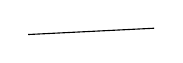
\begin{tikzpicture}\draw (0,0)--(1.6,.08);\end{tikzpicture}}
Jusqu'à présent, on a maintenu $X$, $u$ fixes, on a fait varier $l$, resp. $(T/X,x,y)$. Si on regarde ce qui se passe pour $u\in\Gamma$ variable, les formules
\margin{76}

\scanpage{78}
essentielle triviale, qui fait pendant à (6), est
\[
\tag{28}{}^{uv}l={}^u({}^vl)
\qquad u,v\in\Gamma,\quad l:x\longrightarrow y\quad\text{chemin dans }\unsure{\widehat\Pi_1(X)|\Pi_1(X)}
\]
\deleted{d'où,} si $l$ est chemin de $\Pi_1(X)$, d'où
\[
{}^vl=g_l(v)\cdot l
\]
\deleted{grâce à (6)} d'où on tire par (\unsure{6|8})
\[
{}^u({}^vl)={}^u\{g_l(v)\}\cdot\underbrace{{}^ul}_{g_l(u)\cdot l}
={}^ug_l(v)g_l(u)\cdot l
\]
d'où on tire
\[
\tag{29}\left\{\begin{aligned}
\deleted{\unsure{u}}g_l(uv)&={}^ug_l(v)\cdot g_l(u)\qquad\text{soit}\\
g_l^{-1}(uv)&=g_l^{-1}(u)\cdot{}^ug_l^{-1}(v)
\end{aligned}\right.
\]
Et de $=$
\[
\tag{30}f_l(uv)=f_l(u)\cdot{}^uf_l(v)
\]
i.e. $\unsure{f_{l\alpha}|f_l}$ et $g_l^{-1}$ sont, pour $l$ fixé, $u$ variable, des $1$-cocycles \inserted{sur $\Gamma$} à valeurs dans $\widehat\Pi_1(X,x)$ resp. $\widehat\Pi_1(X,y)$, \inserted{(groupes sur lesquels $\Gamma$ opère)}, d'ailleurs déduits l'un de l'autre par l'isomorphisme
\diagram{\begin{tikzcd}[ampersand replacement=\&]
\widehat\Pi_1(X,x)\arrow[r,"\Pi_1(l)"]\&\widehat\Pi_1(X,y)
\end{tikzcd}}
induit par $l$ \unsure{\ldots\ \deleted{$l$}|\deleted{en $l$}} Ici, c'est la formule pour $f_l$ qui a une gueule plus sympathique que celle pour $g_l$ (pour (10)(11) c'était l'inverse --- \inserted{exprim.} \unsure{``multiplicativité en $l$''}). Les $1$-cocycles obtenus (\deleted{et} $f$ \inserted{un $1$-\unsure{cocycles|cocycle}} droit, $g$ un $1$-cocycle à gauche) correspondent à des $\Gamma$ torseurs à droite resp. à gauche sous $\widehat\Pi_1(X,x)$ resp! $\widehat\Pi_1(X,y)$, qui bien sûr n'est autre que $\operatorname{Hom}_{\widehat\Pi_1(X)}(x,y)$

\margin{On pourrait expliciter \unsure{au demeurant|un de vue qui voit} le couple $(f_l,g_l)$ comme un ``bicocycle'' sur $\Gamma$, relatif à un $\Gamma$-bitorseur $\operatorname{Hom}_{\widehat\Pi_1(X)}(x,y)$ sous $(\widehat\Pi_1(X,y),\widehat\Pi_1(X,x))$}
\margin{77}

\scanpage{79}
\mspage{7}
dont $l$ est justement un élément prenant le rôle d'un ``élément origine'', pour en déduire des $1$-cocycles\ldots

\deleted{Le théorème de Mordell-Weil implique que si $K$ est un corps de type fini sur $Q$, et si $X$ peut se plonger dans une \inserted{VA, ou dans un} groupe algébrique ext. d'une \uline{VA par un tore,} \uline{alors pour $x_0$ fixé,}} \begin{tikzpicture}[baseline=0pt,x=1cm,y=1cm]\draw (0,0) .. controls (-0.015,0.22) and (-0.015,0.45) .. (-0.045,0.65);\end{tikzpicture}

Si on garde $x,y$, et puis remplace $l$ par un $l':x\longrightarrow y$, alors \deleted{\unsure{les|le}} on aura
\[
l'=la=bl\qquad a\in\Pi_1(X,x),\ b\in\Pi_1(X,y)
\]
et on aura, en vertu de (10)(11)
\[
\tag{31}\left\{\begin{aligned}
f_{l'}(u)&=\operatorname{int}(a^{-1})f_l(u)\underbrace{f_a(u)}_{a^{-1}\cdot{}^ua}=a^{-1}\cdot f_l(u)\cdot{}^ua\\
g_{l'}(u)&=\underbrace{g_b(u)}_{{}^ub\cdot b^{-1}}\operatorname{int}(b)\underbrace{g_l(u)}_{\deleted{\unsure{{}^ua\cdot a^{-1}|a^{-1}\cdot{}^ua}}}={}^ub\,g_l(u)b^{-1}
\end{aligned}\right.
\]
\[
(\text{i.e. }g_{l'}^{-1}(u)=b\,g_l^{-1}(u)\,{}^ub^{-1})
\]
\unsure{enfin}, $f_{l'}$ est un $1$-cocycle \inserted{à droite} homologue à $f_l$, $g_{l'}$ un $1$-cocycle \inserted{à g.} homologue à $g_l$. Ainsi, pour $x,y\in X_K$, on trouve des éléments
\[
\tag{32}\left\{\begin{aligned}
g_{y,x}&\in H^1_{\unsure{g}}(\Gamma,\widehat\Pi_1(X,y))\\
f_{y,x}&\in H^1_{\mathrm{dr}}(\Gamma,\widehat\Pi_1(X,x))
\end{aligned}\right.
\]
\deleted{\unsure{donc}} qui sont ``associés'' en un sens convenable, via les isom extérieurs canoniques
\diagram{\begin{tikzcd}[ampersand replacement=\&]
\widehat\Pi_1(X,x)\arrow[r,"\substack{\mathrm{isom}\\\mathrm{ext}\\\sim}"]\&\widehat\Pi_1(Y,y)
\end{tikzcd}}

\margin{Les $f_l(u),g_l(u)$ sont définis, et les formules \unsure{déjà de type|de type} (31) valables, sans \unsure{qu'on exige que} $l:x\unsure{\longrightarrow|\mathbin{-}}y$ provienne de $\Pi_1(X)$, seulement de $\widehat\Pi_1(X)$. Et la définition des classes de $f_{\unsure{l|y}},g_{\unsure{l|y}}$ (ou classes de cohomologie) (32) ne dépend pas des considérations transcendantes, ni de la \unsure{fixation du} corps de base $\mathbb C$\ldots}
\margin{78}

\scanpage{80}
toute la structure étant décrite canoniquement en termes du bitorseur $\operatorname{Hom}_{\widehat\Pi_1(X)}(x,y)$ sous $(\widehat\Pi_1(X,y),\widehat\Pi_1(X,x))$ et l'opération de $\Gamma$ sur \deleted{tout} ce fourbis. On se rappellera surtout que $f_{\unsure{y,x|x,y}}$ et $g_{y,x}$ se déterminent mutuellement, et qu'ils sont déterminés par la connaissance d'\uline{un seul} \deleted{$f_l$ \inserted{$:\Gamma\longrightarrow\widehat\Pi_1(X,x)$} (ou} \deleted{$g_l$ (ie. $f_l(u)$} $f_l$, ou $g_l$
\[
\tag{33}\left\{\begin{aligned}
f_l&:\Gamma\longrightarrow\widehat\Pi_1(X,x)\\
g_l&:\Gamma\longrightarrow\widehat\Pi_1(Y,y)
\end{aligned}\right.
\qquad l:x\longrightarrow y\quad(\text{dans }\Pi_1(X))
\]
(si on a \deleted{\unsure{un}} un $T^\alpha$ $1$-connexe $\subset X$, contenant $x,y$) ils sont connus quand on connaît seulement $g^{T^\alpha}_{x,y}$.

\margin{\uline{NB} $f_{x,y}$ et $f_{y,x}$, ou $g_{x,y}$ et $g_{y,x}$, se déterminent mutuellement, car en termes du chemin $l$, on a p.ex
\[
\tag{34}\left\{\begin{aligned}
g_{l^{-1}}(u)&=f_l(u)^{-1}\\
f_{l^{-1}}(u)&=g_l(u)^{-1}
\end{aligned}\right.
\]}

Quand $X$ se plonge dans une VA, plus généralement s'il se plonge dans une extension d'une VA par un tore (p.ex. $X$ courbe alg. ``anabélienne''), alors le th. de Mordell-Weil implique que pour un $x_0$ \inserted{$\in X_K$} fixé (comme pt de référence --- mais ce $x_0$ \deleted{\unsure{vient}} \unsure{pour|joue} un rôle bidon!)
\margin{79}

\scanpage{81}
\mspage{8}
un point $x\in X_K$ est entièrement déterminé par la connaissance de \deleted{$f_{x_0,x}$}
\[
f_{x_0,x}\in H^1_{\mathrm{dr}}(\Gamma,\widehat\Pi_1\underbrace{(X,x_0)}_{\widehat\Pi(x_0)}),
\]
et a fortiori par la connaissance du \unsure{\inserted{$1$-cocycle}}
\[
f_l:\Gamma\longrightarrow\widehat\Pi^{\unsure{\text{ét}}}(x_0)\qquad\text{pour un seul}
\]
$l:x_0\longrightarrow x$ --- ou ce qui revient au $=$, par la connaissance de $g_{l^{-1}\deleted{\unsure{x_0}}}\in H^1_g(\Gamma,\widehat\Pi_1(x_0))$, \inserted{où $l^{-1}:x\longrightarrow x_0$.}
\margin{$f_l=(g_{l^{-1}})^{-1}$}

\unsure{4|\P} La détermination ``explicite'' d'un $f_l$ --- \deleted{d'un $g_{l^{-1}}$} (qui caractérise donc $x$ dans le cas envisagé) est un pb très intéressant, et sûrement profond. Comme \deleted{\unsure{on} \unsure{un}} \inserted{le} groupe $\Gamma$ bien sûr est loin d'être connu et à la main, il faut préciser d'ailleurs ce qu'on peut bien pouvoir appeler une ``détermination'' (voire dét. explicite!) de $f_l$. Pour ceci, il faut sûrement considérer qu'un $u\in\Gamma$ est repéré par les invariants $f_{l_j}(u)\in\widehat\Pi_1(x_j)$ ou $g_{l_j}(u)\in\widehat\Pi_1(y_j)$, associés plus haut à un système \inserted{fini} de générateurs \inserted{$l_j:x_j\longrightarrow y_j$} du groupoïde $\Pi_1(X,I)$ ($j\in J$, ens d'indices pour les flèches génératrices, $x_j,y_j\in I$),
\margin{80}

\scanpage{82}
\margin{81}
ou de façon équivalente, par les $g^\alpha_{x,y}$ \inserted{$\in\widehat\Pi_\alpha$}, où $\alpha\in A$, $x,y\in I_\alpha$ (cf plus haut). Ceci rappelé,
\margin{\figure{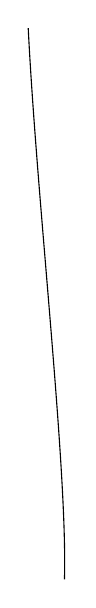
\begin{tikzpicture}\draw (0,0)..controls(.04,1.4)and(-.35,4.8)..(-.46,7);\end{tikzpicture}}}
on peut espérer donner des ``formules'' explicites, \uline{dépendant bien sûr des propriétés arithmétiques précises du point particulier} $x$, et \uline{caractéristiques de} $x$ (dans la situation Mordell-Weil-Néron), qui donnent $f_l(u)$ \uline{en termes} des paramètres précédents fixant $u$. C'est là un travail fascinant en perspective, que je n'ai pratiquement pas amorcé encore pour le moment!

À vrai dire, la démonstration via Mordell-Weil de l'unicité d'un $x$ \inserted{$\in X_K$} qui correspond à une classe donnée dans $H^1(\Gamma,\widehat\Pi_1(x_0))$, montre qu'on a unicité $=$ si on \deleted{\unsure{en donne}} \inserted{\unsure{connait|connaît}} seulement l'élément correspondant à \deleted{\unsure{un}}
\[
\tag{34}(f_{x_0,x})_{\mathrm{ab}}\in H^1(\Gamma,\widehat\Pi_1(X,x_0)_{\mathrm{ab}}),
\]
et on peut déjà essayer de déterminer, par ``formules explicites'', les $(f_l)_{\mathrm{ab}}$ correspondant à des chemins $x_0\longrightarrow x$. On est réduit à regarder la $=$ question en remplaçant $X$ par une VA ou ext. d'icelle,

\margin{(C'est une question particulière, qui \unsure{bien plus intéressante|des plus intéressantes} \illegible{?} \unsure{un problème|une formule} \unsure{variable|valable} \unsure{en} $X$ \unsure{au-dessus de} $\unsure{\mathbb Q}$ \illegible{?}\unsure{.)}}

\scanpage{83}
\mspage{9}
par un tore --- pratiquement, par une ``jacobienne généralisée'' convenable de $X$.

Mais il faut se rappeler que pour une telle variété (p.ex. une courbe elliptique, ou la variété $G_m(\mathbb C)=\mathbb C^*$) l'opération de $\Gamma$ sur le groupoïde $\Pi_1(X_K)$ n'a plus rien de fidèle, donc pour ``repérer'' un $u\in\Gamma$, il ne suffit pas de connaître des invariants du type $g_l(u)$ \uline{relatifs à} \uline{ce même} $X$. Il faudra donc de façon essentielle introduire des ``paramètres de repérage'' pour $u$, en utilisant d'autres variétés algébriques déf sur $K$ --- la plus naturelle étant
\[
\tag{35}\unsure{\mathbb U|U}_{0,3}=\mathbb P^1\setminus\{0,1,\infty\}
\]
\figure{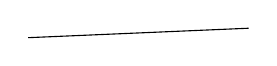
\begin{tikzpicture}\draw(0,0)--(2.8,.12);\end{tikzpicture}}
Faisant maintenant varier $X$, en \unsure{considérant} un morphisme de $K$-schémas
\[
\tag{36}f:X\unsure{\mathbin{-}|\to}X
\]
on déduit des morphismes de groupoïdes
\margin{82}

\scanpage{84}
\diagram{\((37)\)\qquad\begin{tikzcd}[ampersand replacement=\&]\Pi_1(X)\arrow[r,"\unsure{f_*|f}=\Pi_1(f)"]\&\Pi_1(Y)\end{tikzcd}}
\diagram{\((38)\)\qquad\begin{tikzcd}[ampersand replacement=\&]\widehat\Pi_1(X)\arrow[r,"\widehat f=\widehat\Pi_1(f)"]\&\widehat\Pi_1(Y)\end{tikzcd},}
dont le deuxième peut être déduit du premier par passage au groupoïde profini associé, mais peut aussi se décrire directement en termes purement schématiques, en termes \inserted{des morphismes} de schémas \deleted{\unsure{sur|au}} $X\mathbin{-}Y$ sur le corps alg. clos $\mathbb C$. Par suite, (38) commute à l'action de $\mathbf{\Gamma}$,
\[
\tag{39}\widehat f({}^ul)={}^u(\widehat f(l))
\]
et si on se borne aux sous-groupoïdes induits sur $X_{\bar K},Y_{\bar K}$, \inserted{d'où} ($\widehat\Pi_1\,Y_{\bar K}$), ce dernier commute à l'action de $\Gamma=\operatorname{Gal}\bar K/K$. Si on se borne $=$ aux sous-groupoïdes induits $X_K$, d'où des $f_l(u),g_l(u)$ pour un chemin $l$ dans $X$ ou dans $Y$, on trouve aussitôt
\[
\tag{40}\left\{\begin{aligned}
\widehat f(f_l(u))&=f_{\widehat f(l)}(u)\\
\widehat f(g_l(u))&=g_{\widehat f(l)}(u).
\end{aligned}\right.
\]
\margin{Même formule dans le cas d'un $T$ $1$-connexe sur $X$ ($T$ esp. \unsure{topologique}) donc au-dessus de $Y$ On aura:
\[
\tag{40bis}g^{T/Y}_{y,x}(u)=\widehat f(g^{T/X}_{y,x}(u))
\]
\deleted{\unsure{d'où}}}
\margin{83}

\scanpage{85}
\mspage{10}
Un cas trivial intéressant est celui où $f$ est un isomorphisme --- et $=$ celui où $X=Y$, et où $f$ fait partie d'un groupe \inserted{$\mathcal G$} de $K$-isomorphismes de $X$ --- alors on peut considérer $\Pi_1(X)$ et $\Pi_1(X_{\bar K}),\Pi_1(X_K)$ comme des groupoïdes où opère $\mathcal G$, et $\widehat\Pi_1(X)$ comme un groupoïde où opère $\mathcal G\times\mathbf{\Gamma}$, $\widehat\Pi_1(\bar X_{\bar K})$ comme un groupoïde sur lequel $\mathcal G\times\Gamma$ opère. Cette fois-ci le groupe n'opère pas trivialement sur les sommets de $\Pi_1(X_K)$, l'opération de $\Gamma$ est triviale, mais pas nécessairement celle de $\mathcal G$.

Si on se donne un pt $x_0\in X_K$ comme pt base, et un ens de sommets $I\subset X_K$ contenant $x_0$, l'opération de $\Gamma$ sur $\widehat\Pi_1(X,I)$ est connue quand on \unsure{connait|connaît} son opération sur $\widehat\Pi_1(X,x_0)$, et si de plus on \unsure{connait|connaît} son opération sur les $\widehat\Pi_1(X,x_0)$-torseurs ! droit
\figure{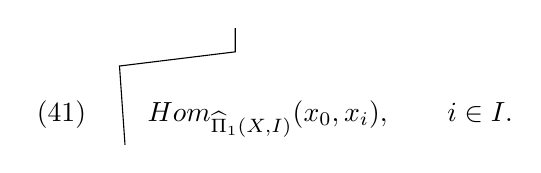
\begin{tikzpicture}
\node[anchor=base east] at(-.65,0) {$(41)$};
\node[anchor=base west,inner sep=0pt] at(0,0) {$\uline{\operatorname{Hom}}_{\widehat\Pi_1(X,I)}(x_0,x_i),\qquad i\in I.$};
\draw(-.28,-.30)--(-.35,.70)--(1.12,.88)--(1.12,1.18);
\end{tikzpicture}}
ou, ce qui revient au $=$, si on connait les
\margin{84}

\scanpage{86}
\[
\tag{41}f_{l_i}(u)\qquad i\in I,\ u\in\Gamma
\]
où pour tt $i\in I$, $l_i$ est un chemin dans $\Pi_1(X,x_i)$ de $x_0$ vers $x_i$, i.e. un élément de la partie ``discrète'' du torseur (41).

D'autre part, l'action de $\Gamma$ sur $\widehat\Pi_1(X,x_0)$ est connue quand on \unsure{connait|connaît} son action sur des générateurs $\lambda_j$ \inserted{($j\in J$)} de $\Pi_1(X,x_0)$, ie. si on \unsure{connaît|connait} les
\[
\tag{43}f_{\lambda_j}(u)\quad\text{ou}\quad g_{\lambda_j}(u)\qquad j\in J,\ u\in\Gamma.
\]
\deleted{Mais cette} Les données (42)(43) suffisent donc à déterminer l'action de $\Gamma$ sur $\Pi_1(X,I)$ --- mais cette description, \deleted{à la} \deleted{dis} s'il a l'avantage d'une économie, au moins en apparence, a le désavantage de se référer à des choix arbitraires, le pire étant le choix \unsure{d'un|d'une} \deleted{origine} \inserted{point-base} $x_0$ \deleted{à laquelle} \inserted{auquel} on est censé tout ramener --- ce qui semble artificiel, et à la longue je crois impraticable, \deleted{\unsure{et|est}} et tout particulièrement dans les situations impliquant un groupe de \unsure{symétrie|symétries} $\mathcal G$ comme ci-dessus, quand on a pris $I$ stable sous $\mathcal G$ ---
\margin{qu'il faut \unsure{exprimer} \unsure{linéairement|littéralement}, \unsure{resp.|resp} principe, \unsure{décrit p.8!|dit p.8'}}
\margin{85}

\scanpage{87}
\mspage{11}
alors que pratiquement jamais on ne pourra trouver un $x\in X_K$ \deleted{stable} \inserted{fixe} sous $\mathcal G$.
\figure{\begin{tikzpicture}\draw (0,0)--(1.4,0);\end{tikzpicture}}

Avant de donner un principe d'approche pour des calculs ``symétriques'', tenant compte de la présence d'un groupe $\mathcal G$ (cas d'une grande importance en pratique), je 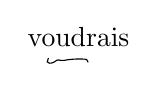
\begin{tikzpicture}[baseline=(w.base)]\node[inner sep=0pt,outer sep=0pt] (w) {voudrais};\draw ([xshift=.75em,yshift=-.4em]w.south west) -- ++(-.015,-.05) .. controls +(.03,-.04) and +(-.02,-.02) .. ++(.12,.02) .. controls +(.03,.02) and +(-.04,-.02) .. ++(.10,0) .. controls +(.06,.015) and +(-.05,.015) .. ++(.28,.01) -- ++(.02,-.035);\end{tikzpicture} préciser la question de la relation entre $\Pi_1(X,I)$ ($I$ partie finie de $X_K$) et $\Pi_1(U_{0,3})$, \deleted{et les} dans l'optique des opérations de $\Gamma$.
\inserted{Pour fixer les idées je suppose que $K$ est \deleted{\unsure{de}} fini sur $\mathbb Q$,} \inserted{et} Je prendrai le cas $X$ quasi-projective lisse géom.$^t$ connexe. Utilisant des th. du type Lefschetz, plus le résultat de \deleted{Biel} Белый, on \deleted{\unsure{trouve|trouver}} doit pouvoir trouver deux hom de schémas sur $K$
\diagram{\((44)\)\qquad\begin{tikzcd}[ampersand replacement=\&]
I \arrow[d,phantom,"\cap" description] \& \\
\unsure{\mathcal C|C} \arrow[r,hook,"i"] \arrow[d,"f"'] \& X \\
U_{0,3} \&
\end{tikzcd}}
où $i$ induit un hom \uline{surjectif} sur les groupes fondamentaux, et où $f$ est
\margin{86}

\scanpage{88}
un morphisme fini étale. Ainsi $\Pi_1(X,I)$ apparait comme quotient de $\Pi_1(C\deleted{\unsure{X}},I)$, donc $\widehat\Pi_1(X,I)$ quotient de $\widehat\Pi_1(C,I)$, et où $\Pi_1(C,I)$ apparait comme un revêtement fini de $\Pi_1(U_{0,3},I)$ --- plus \deleted{précisément} \inserted{\unsure{concretement|concrètement}}, prenant le saturé $I'=f^{-1}f(I)=f^{-1}(I_0)$ de $I$, $\Pi_1(U_{0,3};I)$ est un sous-groupoide \inserted{plein} de $\Pi_1(U_{0,3};I')$, qui lui est un rev. fini du groupoïde $\Pi_1(U_{0,3};I_0)$ --- et idem pour les complétés profinis. Ainsi, l'opération de $\Gamma$ sur $\widehat\Pi_1(X)$ est connue quand on \unsure{connait|connaît}\unsure{:} l'opération sur $\widehat\Pi_1(C,\widetilde I)$, qui est un rev. fini de $\widehat\Pi_1(U_{0,3};I_0)$. Si on connait l'action de $\Gamma$ sur $\widehat\Pi_1(U_{0,3};I_0)$ lui-même, \deleted{\unsure{La} on doit pouvoir} \inserted{\unsure{l'action|l'opération} sur $\deleted{\widehat\Pi_1(U_{0,3})}$}
\margin{87}

\scanpage{89}
\mspage{12}
$\widehat\Pi_1(C,I')$ est \unsure{déterminée|déterminé} \inserted{via (39) ou (40)}, car l' pour $x,y\in C$, l'application
\[
\operatorname{Hom}_{\widehat\Pi_1(C)}(x,y)\longrightarrow\operatorname{Hom}_{\widehat\Pi_1(U_{0,3})}(\unsure{m|x},y)
\]
est injective!

J'avais pas observé, car le saturé $I'$ de $I$ \inserted{dans $C$} n'est pas tjrs \deleted{fini} contenu dans \deleted{$\unsure{X}$} $C_K$ --- mais à vrai dire, rien ne m'obligeait à remplacer $I$ par $I'$ pour faire mon raisonnement: il reste vrai que la connaissance de l'action de $\Gamma$ sur sur $\widehat\Pi_1(U_{0,3},I_0)$ implique la connaissance de son action sur $\widehat\Pi_1(X,I)$. Mais il est vrai sûrement que l'étude des relations entre $\widehat\Pi_1(C;\deleted{\unsure{x}}I)$ et $\widehat\Pi_1(U_{0,3},I_0\unsure{)}$ en tant que groupoïdes à groupe d'opérations $\Gamma$, est facilité grandement en remplaçant $I$ par son saturé $I'$, $=$ si celui-ci n'est pas $\subset\deleted{X}C_K$. (Au besoin, si on est ennuyé par des sommets qui se balladent sous l'action de $\Gamma$, il n'y a
\margin{88}

\scanpage{90}
\margin{89}
qu'à remplacer $\Gamma$ par un sous-groupe ouvert convenable $\Gamma'$\ldots)

En $=$ temps, on entrevoit des conditions nécessaires draconiennes pour qu'un autom. \inserted{$\Theta$} du groupoïde $\Pi_1(U_{0,3};I_0)$, laiss.$^t$ fixe les sommets i.e. les pts de $I_0$, provienne d'un $u\in\Gamma$: il faut que pour tt revêtement \deleted{de $X$} étale $C$ de $U_{0,3}$, défini sur $K$, \inserted{prenant $I=f^{-1}(I_0)\subset C_K$ et \unsure{projetant|\deleted{supposant}} $I\to I_0$, \unsure{surj.|surj}} \deleted{telle que} \deleted{l'action de} \deleted{\unsure{l'opération de}} \inserted{que l'autom.} $\Theta\deleted{_{C_0}}$ \deleted{de} $\Pi_1(U_{0,3},I_0)$ \deleted{provienne d'une action de} \inserted{soit ``compatible'' avec un autom.} $\Theta_C$ de $\Pi_1(C,I)$ \inserted{qui soit l'identité} \deleted{\unsure{qui soit ponctuel|qui soit ponctuellement}} \inserted{sur les sommets $I$} \deleted{par l'identi} (cet $\Theta_C$ sera alors unique). On trouve encore une condition, $=$ si $I-I_0$ n'est pas surjectif, et sans supposer $=$ que $I_0\subset \deleted{\unsure{U}}\inserted{C}_{0K}$ pour $\unsure{\forall|\mathrm{tt}}$ rev. étale de $U_{0,3}$, en exigeant qu'il existe une puissance \inserted{$\Theta^n$} de $\Theta$ \inserted{($n\geq1$)} satisfaisant aux conditions précédentes, pour $I=f^{-1}(I_0)$ \unsure{---|.}
\margin{(NB $C_0=U_{0,3}=P^1_{\mathbb C}\setminus\{0,1,\infty\}$)}
\margin{Regarder des \unsure{familles} \illegible{2} \deleted{\unsure{telles}} \unsure{conditions} \unsure{de} \illegible{1}, quand on augmente $I_0$\ldots}

\scanpage{91}
\mspage{13}
Non seulement la condition d\unsure{é|e} \deleted{continuité} ``prolongeabilité'' --- il vaut mieux dire d'inductibilité'' --- sous la forme précisée, ou affaiblie (avec $\Theta$ remplacé par un $\Theta^n$), on trouve une condition supplémentaire, quand on a \inserted{de plus} un morphisme
\[
\widehat\Pi_1(C,I)\longrightarrow\widehat\Pi_1(X,I),
\]
que celui-ci passe au quotient --- ce qui s'exprime très exactement par la condition que pour \uline{un} $x_0\in I$, l'action de $\Gamma$ sur
\[
\widehat\Pi_1(C,x_0)\subset\widehat\Pi_1(U_{0,3},f(x_0))
\]
laisse stable le noyau de
\[
\widehat\Pi_1(C,x_0)\longrightarrow\widehat\Pi_1(X,x_0);
\]
alors ce sera vrai également pour tous les autres $x_i\in I$.

Il faut exprimer la possibilité de relever l'action \deleted{de} $\Theta$ à $\Pi_1(C,I)$. Notons à ce propos

\uline{Lemme} Soit $\mathcal C'\unsure{\mathbin{-}|\to}\mathcal C$ un hom de groupoïdes connexes, qui soit injectif sur les $\Pi_1$, \unsure{\deleted{et}|(} de sorte que $\mathcal C'$ est équivalent à un revêtement de $\mathcal C$, mais on ne suppose pas que $\mathcal C'$ soit lui-$=$ un revêtement de $\mathcal C$, mais quand-même que
\margin{90}

\scanpage{92}
l'homomorphisme canonique
\[
\tag{45}\mathcal C'\longrightarrow\widetilde{\mathcal C}^{\unsure{\prime|*}}.
\]
\inserted{vrai revêtement de $\mathcal C$, dont les sommets sont les $\pi_0$ des fibres de $\mathcal C'\mathbin{-}\widetilde{\mathcal C}^{\unsure{*|\prime}}$}
\deleted{\unsure{soit}} factorisant $\mathcal C'\mathbin{-}\mathcal C$ est injectif, de sorte qu'on peut identifier $\mathcal C'$ à un sous-groupoïde plein de $\widetilde{\mathcal C}^{*}$, équivalent à $\widetilde{\mathcal C}^{*}$ par l'inclusion, où $\widetilde{\mathcal C}$ est un rev. fini de $\mathcal C$\unsure{.}

Soit $x'_0$ un sommet de $\mathcal C'$, $x_0$ son image dans $\widetilde{\mathcal C}$. Soit $\Theta$ un automorphisme de $\mathcal C$ qui fixe $x_0$, \deleted{alors s'}il \deleted{\unsure{y en a un de}\unsure{.}} \inserted{revient au} $=$ de se donner un autom. de \deleted{$\mathcal C$} $\Pi_1(\mathcal C,x_0)\overset{\mathrm{def}}{=}\Pi_0$ (\unsure{abrég.}), et pour tout \inserted{sommet} $\deleted{\unsure{x}}x_i\in\operatorname{Ob}\mathcal C$, $x_i\ne x_0$, un automorphisme du $\Pi_1(x_0)$-torseur à droite $H_{x_i,x_0}=\operatorname{Hom}_{\mathcal C}(x_0,x_i)$, compatible avec l'opération de $\Theta$ sur $\Pi_0$. Ceci posé, pour que cette action se remonte en une action de $\widetilde{\mathcal C}$ qui fixe $x'_0$, il f et s. que le sous-groupe $\Pi'_0$ de $\Pi_0$, image de \deleted{$\unsure{\Pi_1(}$}
\[
\Pi_1(\widetilde{\mathcal C},x'_0)\hookrightarrow\Pi_1(\mathcal C,x_0)=\Pi_0,
\]
soit \uline{stable} par $\Theta$ --- l'action de $\Theta$ sur les fibres \inserted{$\widetilde{\mathcal C}_{x_i}$} de $\widetilde{\mathcal C}/\mathcal C$ est alors donnée par la formule
\[
\tag{45}\operatorname{Ob}\widetilde{\mathcal C}_{x_i}=H_{x_i,x_0}\wedge_{\Pi_0}\underbrace{\Pi_0/\Pi'_0}_{\substack{\text{\unsure{espace|esp.} \unsure{hom|hom.}}\\\text{des classes}\\\text{à droite, sur lequel}\\\Pi_0\ \text{opère à \unsure{g|g.}}}}
\]
par transport de structure : partir de son
\margin{91}

\scanpage{93}
\mspage{14}
action sur \deleted{$H_{x_i,x_0}$} le système $(\Pi_0,H_{x_i,x_0},\underbrace{\Pi_0/\Pi'_0}_{\deleted{\unsure{esp|espace}}})$ où on fait opérer $\Theta$ sur $\Pi_0,H_{(x_i,x_0)}$ par son action sur $\mathcal C$, et sur $\Pi_0/\Pi'_0$ via l'action sur $\Pi_0$, qui passe au quotient d'après la \deleted{hypothèse} \inserted{condition} \deleted{dite} envisagée. L'action \deleted{prolong} remontée \inserted{$\unsure{\widetilde\Theta|\Theta'}$ de $\Theta$} \deleted{est} sur $\widetilde{\mathcal C}$ est donc unique. Pour qu'il existe une action de $\Theta^{*}$ sur $\mathcal C'$ qui soit compatible avec $\mathcal C'-\mathcal C$, il f. et s. que la condition précédente soit satisfaite, et que \uline{de plus} $\operatorname{Ob}\mathcal C'\subset\operatorname{Ob}\mathcal C$ soit stable sous \deleted{cette} l'action de $\widetilde\Theta$.

Dans le cas où on ne suppose pas que l'on \deleted{dispose de} \inserted{donne} un $x'_0\in\operatorname{Ob}\mathcal C'$ dont on exige qu'il soit fixe par $\Theta$, on considère la fibre \inserted{$E_0=$} $\widetilde{\mathcal C}_{x_0}$, qui est un $\Pi_0$-ensemble \deleted{\unsure{un}} homogène, et on note que les façons de remonter $\Theta$ en une action \inserted{$\unsure{\overline\Theta|\widetilde\Theta}$} dans $\widetilde{\mathcal C}$ correspondent \deleted{\unsure{aux}} exactement aux façons de remonter $\Theta$ en une action de $\widetilde\Theta_0$ sur $E_0$, \deleted{\unsure{comment|convenant}} soit compatible avec l'action sur $\Pi_0$, i.e satisfaisant
\margin{mais on suppose tjrs un $x_0$ fixe sous $\Theta$}
\figure{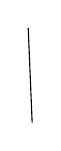
\begin{tikzpicture}\draw(0,0)--(-.05,1.2);\end{tikzpicture}}
\margin{Ceci vaut sans supposer $\widetilde{\mathcal C}$ connexe --- mais la traduction plus bas en termes de $\Pi'_0\subset\Pi_0$ dépend de la condition de connexité.\ldots Cf plus bas le cas où on a un \unsure{s-grp} plein $\mathcal C$ connexe}
\[
\tag{46}\widetilde\Theta_0(g.x^{\deleted{\unsure{0}}\prime})\mathord{\hbox{\begin{tikzpicture}[baseline=0pt]\path[use as bounding box] (-.015,0) rectangle (.05,.28);\fill (0,.19) circle[radius=.010];\fill (.035,.26) ellipse[x radius=.010,y radius=.014];\end{tikzpicture}}}=\Theta(g)\widetilde\Theta_0(x')
\]
--- \deleted{elle correspond} \inserted{une telle action} est connue quand on \unsure{connait|connaît}, pour \uline{un} $x'_0$ fixé de $E_0=\operatorname{Ob}\widetilde{\mathcal C}_{x_0}$, son transformé par $\widetilde\Theta_0$, la formule (46) donnant tous les autres \inserted{$\widetilde\Theta_0(x')$, \deleted{puisque $\unsure{x'\in E_0}$} $\unsure{\mathrm{pr}|\forall}\,x'\in E_0$}. En termes
\margin{92}

\scanpage{94}
de $\Pi_0$, $\Pi'_0=\operatorname{Im}(\Pi_1(\widetilde{\mathcal C},x'_0)\mathbin{-}\Pi_1(\mathcal C,x_0))$, de sorte que \deleted{$\unsure{\widetilde{\mathcal C}|\widetilde E}$}
\[
\unsure{(47)|47)}\qquad E_0\simeq\Pi_0/\Pi'_0;
\]
la condition d'existence de $\widetilde{\Theta}_0$ revient à dire
\[
\Theta(\Pi'_0)\text{ conjugué à }\Pi'_0\text{ dans }\Pi_0
\]
\margin{en effet, il faudra que $\Theta(\Pi'_0)$ soit $\operatorname{Im}(\Pi_1(\widetilde{\mathcal C},x'_1)\unsure{\mathbin{-}|\to}\underbrace{\Pi_1(\mathcal C,x_0)}_{\Pi_0})$, où $x'_1=\widetilde{\Theta}(x'_0)$, Or si $x'_1=g(x'_0)$, où $g\in\Pi_0$, l'Im en question vaut $\operatorname{int}(g)(\Pi'_0)$}
et les choix possibles pour remonter $\Theta$ en $\widetilde{\Theta}_0$, donc pour remonter $\Theta$ en $\widetilde{\Theta}$, correspondent aux éléments \inserted{$\unsure{x'_1|x''}$} de $E_0$ \deleted{tels que} \inserted{de la} forme $g(x'_0)$ avec $g\in\Pi_0$ satisfaisant
\[
(48)\quad\unsure{;|:}\qquad \operatorname{int}g(\Pi'_0)=\Theta(\Pi'_0)
\]
i.e. tels que
\[
g\in\operatorname{Transp}_{\Pi_0}(\Pi'_0,\Theta(\Pi'_0))
\]
\margin{Cette condition ne dépend que de l'endom \uline{ext.} défini par $\Theta$ sur $\Pi'_0$ --- mais la façon de remonter $\Theta$ en $\widetilde{\Theta}$, $=$ comme endom ext, en dépend, \unsure{aux de l'} \uline{pas} \unsure{un|en} endom. ord. \unsure{défini} par $\Theta$}
\margin{\deleted{\unsure{pts} \illegible{2}}\quad\deleted{\unsure{Si} $\unsure{\widetilde{\mathcal C}}$ \unsure{correspond} \illegible{3} \unsure{on a} $\unsure{\Theta'_0}$ \illegible{3} $\unsure{\Theta}$ \illegible{2} $\unsure{\widetilde{\Theta}}$ \unsure{tel que} $\unsure{E_0}\ \unsure{\exists\gamma\in\Pi_0}$ \unsure{avec} $(48\,\mathrm{bis}):\ \Theta(\Pi'_0)=\gamma(\Pi'_0)$ dans $\Pi'_0$.}}
donc les $\unsure{\widetilde{\Theta}|\Theta}$ possibles correspondent aux éléments de
\[
(49)\qquad \operatorname{Transp}_{\Pi_0}(\Pi'_0,\Theta(\Pi'_0))/\Pi'_0
\]
\margin{espace homogène à droite ($\Pi'_0$ opère à droite sur le transporteur, via $g\longmapsto g\alpha$ pour $\alpha\in\Pi_0$}
\margin{Bien sûr, les façons de remonter $\Theta$: $\Theta'$ de $\mathcal C'\subset\widetilde{\mathcal C}$ correspondent aux $\widetilde{\Theta}$ qui rendent bien ainsi $\mathcal C'\subset\widetilde{\mathcal C}$ invariant.}

Ainsi, on voit que dans le cas \deleted{$\unsure{\mathcal C|\widetilde{\mathcal C}}$}
\[
\mathcal C=\widehat{\Pi}_1(X\deleted{_{\unsure{\overline{k}|\overline K}}},I),\qquad I\subset X_{\unsure{k|K}}
\]
quand $\mathcal C'$ \deleted{en premier} est de la forme $\widehat{\Pi}_1(X'\deleted{_{\unsure{\overline{k}|\overline K}}},I')$, où $X'$ est un rev. étale (fini) de $X$, \inserted{avec $I'\unsure{\mathbin{-}|\to}I$}, que la condition qu'un \inserted{\unsure{endom}} $\Theta$ \inserted{de $\mathcal C$} se remonte en un autom de $\mathcal C'$ est une condition algébrique des plus
\margin{93}

\scanpage{95}
\mspage{15}
\deleted{plus} simples, \unsure{qui|que} pour $I'=p^{-1}(I)$ ne dépend pas du choix de $I'$ i.e. de $I$. Si on veut que l'action remontée $\Theta'$ soit l'identité sur $I'$, on a unicité, et la condition supplémentaire que $\widetilde{\Theta}$ doit bien opérer \uline{trivialement} sur $I'$.

Revenons : l'action de $\Gamma$ \inserted{$=\operatorname{Gal}\overline{K}/K$} sur un $\mathcal{C}=\deleted{\unsure{\Pi_1}}\widehat{\Pi}_1(X,I)$ avec $I\subset X_K$, on trouve donc une condition nécessaire pour qu'un autom $\Theta$ de $\mathcal{C}$ \inserted{trivial sur les objets} provienne d'un $u\in\Gamma$:

\margin{Ces deux conditions ne dépendent en fait que de l'opération de \deleted{$\Theta$} $\Theta$ sur le groupe fondamental en \uline{un} point $x_0\in I$}
a) Pour tout rev. \inserted{étale} fini $X'$ de $X$, \inserted{(défini sur $K$)} \deleted{\unsure{il considère}} \deleted{\unsure{il y a} l'action de} \inserted{il y a une action $\widetilde{\Theta}$ de} $\Theta$ sur $\widehat{\Pi}_1(X',I')$, où $I'=X'|I$, qui remonte $\Theta$, et qui est l'identité sur $I'\cap X'_K$.

b) De plus, pour $\forall$ hom. (défini sur $K$)
\[
X'\xrightarrow{f}Y,
\]
et tout $x'\in I'\cap X'_K$, le noyau de
\[
(*)\qquad\widehat{\Pi}_1(X',x')\longrightarrow\widehat{\Pi}_1(\unsure{Y|X},f x')
\]
est stable sous $\widetilde{\Theta}^{\unsure{\prime|*}}$ \inserted{(pour $\widetilde{\Theta}$ convenable!)} --- plus généralement, sans supposer $x'\in X'_K$, mais choisissant $\nu\in\mathbb{N}^{+}$ tel que $\Theta^\nu x'=x'$, il faut que \deleted{$\Theta$} le noyau de $(*)$ soit stable par $\Theta^\nu$.

\margin{\uline{NB} Ces conditions \deleted{\unsure{de}} informulables, tant que nous \unsure{bornions|bornons} au point de vue des actions \uline{extérieures} de $\Gamma$!}
\figure{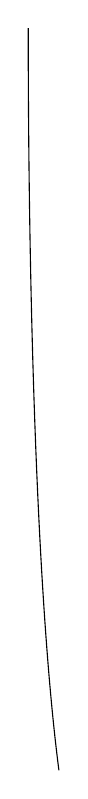
\begin{tikzpicture}[x=0.01cm,y=0.01cm]
\draw (0,0) .. controls (0,-320) and (10,-720) .. (39,-943);
\end{tikzpicture}}
Ce sont là des conditions draconiennes. Je \unsure{pense|peux} que ce n'est pas trop m'avancer,
\margin{94}

\scanpage{96}
en conjecturant que ces conditions \inserted{nécessaires} sont suffisamment draconiennes \deleted{pour} (même sans entrer ds la considération des $\Theta^\nu$) pour assurer que $\Theta$ provient bien d'un $u\in\Gamma$, \deleted{lors} lorsque $X$ est (disons) une \uline{courbe algébrique anabélienne}, avec extension de type fini de $\mathbb{Q}$.
\margin{Je ne vois pas très bien si la condition a), sans b), devrait être suffisante pour assurer que $\Theta$ vient de $\Gamma$. Et puis, \unsure{en} tous ces \unsure{autres}, et pour les groupes profinis...}
\margin{
\figure{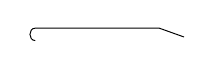
\begin{tikzpicture}[x=.45cm,y=.45cm]
\draw[line width=.35pt] (0,-.35) .. controls (-.2,-.35) and (-.2,0) .. (0,0) -- (3.5,0) -- (4.2,-.25);
\end{tikzpicture}}
\deleted{on \unsure{peut}} pas évident que l'hypothèse anabélienne soit requise --- à examiner! (\unsure{N'est} \illegible{?} pour $\mathbb{G}_m$, ou une courbe elliptique). La variation : $X/K$ de dim $1$ me semble également inessentielle. En fait, c'est faux pour $\mathbb{G}_m$
\figure{\begin{tikzpicture}[x=.45cm,y=.45cm]
\draw[line width=.35pt] (0,0) -- (4.2,0) -- (4.2,.35) -- (5.15,.35);
\end{tikzpicture}}
}
\figure{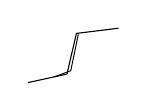
\begin{tikzpicture}[x=.6cm,y=.6cm]
\draw[line width=.4pt] (0,0) -- (.82,.18) -- (1.02,1.04) -- (1.91,1.15);
\draw[line width=.35pt] (.55,.12) -- (.9,.25) -- (1.06,1.02);
\end{tikzpicture}}
Bien sûr, la question de l'unicité de $u$ n'est pas impliquée ici --- quand $K$ est une extension algébrique de $\mathbb{Q}$, on s'attend à l'\uline{unicité} de $u$. Quand $K$ est de degré de transcendance $>0$, alors pour pouvoir s'attendre à l'unicité de $u$, il faut au moins supposer que le corps modulaire de $X$ a $=$ degré de transcendance, i.e. que $K$ est une extension \uline{finie} de ce corps modulaire. Je ne serais pas étonné qu'on ait unicité dans ce cas.
\margin{Ça doit même pouvoir se démontrer avec ce que je sais, \unsure{i.e.} via Белый. Pour l'unicité, bien sûr, la condition anabélienne est absolument essentielle...}

Je reviens sur la question de la relevabilité d'un \deleted{$\Theta$} endomorphisme $\Theta$ d'un groupoide connexe $\mathcal{C}$ à un revêtement $\widetilde{\mathcal{C}}$, quand $\Theta$ fixe un sommet
\margin{95}

\scanpage{97}
\mspage{16}
$x_0$ de $\mathcal C$, mais sans supposer maintenant $\widetilde{\mathcal C}$ connexe. (\deleted{\unsure{En}} Revenant au cas où $\widetilde{\mathcal C}$ proviendrait d'une situation géométrique $X'\mathbin{-}X$, avec $X$ connexe, \deleted{et un \unsure{revêtement}} mais $X'$ seulement $K$-connexe i.e. connexe en tant que schéma sur $K$ --- ce qui signifie qu'il \deleted{\unsure{p}} se décrit en termes galoisiens par $E_0=X'_{x_0}$, sur lequel le produit $\frac12$ direct $\Gamma.\Pi_0$ ($\Pi_0=\Pi_1(X,x_0)=\Pi_1(\mathcal C,x_0)$) opère transitivement, mais sans que l'opération de $\Pi_0$ soit forcément transitive.) Associons à $\forall\ x'\in E_0$ son stabilisateur dans $\Pi_0$, on trouve une application
\diagram{\((50)\qquad
\begin{tikzcd}[ampersand replacement=\&,column sep=large,row sep=small]
E_0 \arrow[r] \& \text{Ens des ss-groupes de }\Pi_0 \\
x' \arrow[r,mapsto] \& \text{stabilisateur }\Pi_{\unsure{0x'|x'}}
\end{tikzcd}\)}
qui commute aux actions de $\Pi_0$ (op. sur le $2^e$ ens par autom. intérieurs), d'où par passage aux quotients
\diagram{\((51)\qquad
\begin{tikzcd}[ampersand replacement=\&,column sep=large]
E_0/\Pi_0\overset{\mathrm{def}}=\{\pi_0\}(E_0) \arrow[r,"{\overline{\Sigma}:}"{pos=.85}] \& \operatorname{Ssgr}(\Pi)/\Pi
\end{tikzcd}\)}
\inserted{$\unsure{\deleted{\pi}|\#}$ c'est le $\pi_0$ dans le topos des $\Pi$-ens.}

D'autre part, $\Theta$ opère sur le $2^{\text{ième}}$ mb de (51) par transport de structure, via l'autom donné de $\Pi$, et \unsure{la|\deleted{la}} une condition nécessai-
\margin{96}

\scanpage{98}
évidente pour que $\Theta$ se relève en un $\widetilde{\Theta}$, c'est que l'image de l'application (51) soit \uline{stable} sous l'action de $\Theta$; en fait, l'action $\widetilde{\Theta}$ présomptive, restreinte à $E_0$, doit donner la compatibilité. \deleted{\unsure{Rien qu'en} \illegible{?} Inversement} \inserted{On voit donc qu'en deux pts de $\overline{\Sigma}$ conjugués sous $\Theta$, le degré de (52) (cardinal de la fibre) doit} \deleted{de stabilité} \deleted{telle} que je viens d'énoncer signifie justement qu'il existe une \deleted{$\unsure{\widetilde{\Theta}|\widetilde{\Theta}_0}$} \inserted{bijection}
\margin{\unsure{On l $=$.|On lie} les deux conditions}
\[
(52)\qquad \pi_0(\widetilde{\Theta}_0):\pi_0(E_0)\overset{\sim}{\unsure{\longrightarrow|\mathbin{-}}}\pi_0(E_0)
\]
\deleted{telle que} qui soit compatible avec l'action de $\Theta$ sur le deuxième mb de (51). Ceci dit, pour \unsure{toute telle} relèvement, il existe bel \inserted{\unsure{p.e.|i.e.}} \uline{et} bien un $\widetilde{\Theta}$ qui l'induise, \inserted{$\widetilde{\Theta}_0:E_0\overset{\sim}{\unsure{\to|\mathbin{-}}}E_0$ \deleted{\unsure{qui soit}} compatible avec l'action de $\Pi$ et l'action de $\Theta$ sur $\Pi$ (cf (46))} lequel $\widetilde{\Theta}$ est bien connu quand on connait ses valeurs $\widetilde{\Theta}(x_i)$ \deleted{\unsure{pour}} pour \uline{un} $x_i\in$ \deleted{\unsure{de}} \inserted{$E_0$} dans chaque composante connexe de $E_0$ \ldots

Parmi ces conditions nécessaires \inserted{importantes} sur un automorphisme $\Theta$ d'un $\widehat{\Pi}_1(X,I)$, $I\subset X_K$, pour provenir de $\Gamma$, j'ai oublié apparemment la plus importante de toutes, avec laquelle je travaille \unsure{pourtant|\deleted{pourtant}} constamment --- à tel point qu'elle finit par sembler aller de soi!
\margin{97}

\scanpage{99}
\mspage{17}
C'est la condition de compatibilité avec la ``structure à lacets'' --- dans le cas où $X$ est une courbe algébrique, disons (sinon, on sent bien qu'il faut introduire, dans le cas général, une ``structure à l'infini'' du groupoïde fondamental \ldots). \margin{$\Vert$} Cette compatibilité \inserted{justement} s'exprime de façon particulièrement naturelle et élégante dans le contexte des groupoïdes, \unsure{$\{$} comme une condition de la nature d'une compatibilité à des morphismes de schémas (cf (39)) --- mais on pourrait ici non des schémas de t.f. mais des schémas locaux épointés ou ``rondelles'' épointées --- je vais revenir sur ce point de vue plus bas.

\uline{Remarque.} Revenant aux conditions a) b), il est clair d'emblée qu'elles sont indéchiffrables \inserted{(i.e. inexprimables)} en termes $\pm$ directs, comme des conditions portant directement sur les ``paramètres'' du type $g_{\unsure{\ell|e}}(u)$ \unsure{$\{$|(}des paramètres \deleted{\unsure{comme}} \inserted{tels que} ceux désignés par $\alpha,\beta,\xi,\eta$ dans mon étude des autom. à lacets de $\Pi_{03}$ \ldots) qui ``répèrent'' un $u\in\Gamma$ (ici $\Gamma=\operatorname{Gal}\overline{\mathbb{Q}}/Q$). \deleted{Pourtant} C'est pour cette raison que le
\margin{98}

\scanpage{100}
conjecture énoncée plus haut (que ces conditions, plus la condition des lacets, \inserted{si on veut} sont suffisantes) n'est pas bien intéressante, de nature trop platonique. Mais \unsure{il|je} \deleted{\unsure{paraît}} \inserted{me} semble que via l'étude des multiplicités MD $M_{g,\nu}$ et des groupes de Teichm\unsure{û|ü}ller, je suis en train de me rapprocher du point où une conjecture intéressante et plausible, en termes de propriétés internes des groupes profinis tels que $\widehat{\Pi}_{0,3}$, finira par apparaître, (en commençant par des conditions liées aux $M_{0,4},M_{0,5}\ldots$).
\margin{En un sens, elle met la charrue avant les bœufs --- puisque je cherche à déterminer $\Gamma$ par conditions de nature algébriques, qui ne parlent que des \uline{\unsure{opérations|orientations}} (\unsure{sur} un ensemble) \unsure{du} \unsure{groupoïde} fondamental $\widehat{\Pi}_1(X_{\unsure{K}})$ \unsure{purement|seulement}\ldots}

Je passe en revue encore une fois, sous forme complétée, les conditions pour un automorphisme \inserted{$\Theta$} d'un groupoide $\widehat{\Pi}_1(X,I)$, $I\subset X_{\overline{K}}$, \inserted{$I\cap\unsure{X_{\overline{K}}|X_K}\ne\varnothing$} (je pense surtout, pour le moment, au cas $X=U_{0,3}$) provienne d'un $u\in\Gamma=\operatorname{Gal}\overline{K}/K$:

1) Condition des lacets (pour mémoire --- c'est sûrement la plus importante de toutes, de très loin!)

2) Condition de Stabilité pour revêtements étales \deleted{de} $X'$ de $X$ (définis sur $K$, bien sûr);
\margin{99}
